\section{Curves Defined by Parametric Equations}
  Suppose that $x$ and $y$ are both given as functions of a third variable $t$ (called a \textbf{parameter} by the equations)
    $$ x = f(t) \ \ \ y = g(t) $$
  (called \textbf{parametric equations}). Each value of t determines a point (x,y). As t changes, $ (x,y) = (f(t),g(t)) $ changes and traces out a curve $C$, which is called a \textbf{parametric curve}. The direction of the arrows on curve $C$ show the change in the position of the equation as $t$ increases.

  We can also restrict $t$ to a finite interval. In general, the curve with parametric equations
    $$ x = f(t) \ \ \ y = g(t) \ \ \ a \leq t \leq b $$
  has \textbf{initial point} $(f(a),g(a))$ and \textbf{terminal point} $(f(b),g(b))$.

  \subsection*{The Cycloid}
    \begin{center}
      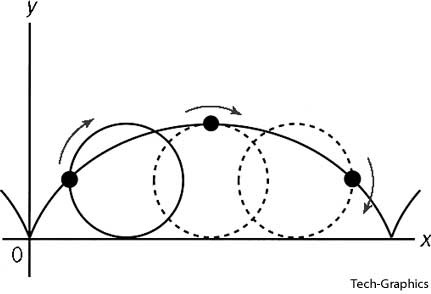
\includegraphics[width=150pt]{cycloid_example.jpg}
    \end{center}
    \begin{example}
      A circle with radius $r$ rolls along the $x$-axis. The curve traced out by a point $P$ on the circumference of the circle is called a \textbf{cycloid}. Find parametric eqations for the cycloid.
    \end{example}
    \begin{solution}
      We will use the angle of rotation $\theta$ as the parameter ($\theta = 0$ when $P$ is at the origin).
      \begin{center}
        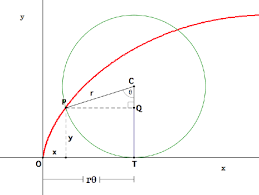
\includegraphics[width=150pt]{cycloid_solution.png}
      \end{center}
      Suppose the circle has rotated $\theta$ radians. Using the figure, the distance it has rolled from the origin is
        $$ |OT| = arc\ PT = r\theta$$
      because P starts at the origin. Therefore, the center of the circle is $C(r\theta,r)$. Let the coordinates of $P$ be $(x,y)$. Then from the figure,
      \begin{align*}
        x &= |OT| - |PQ| = r\theta - r\sin\theta = r(\theta-\sin\theta)\\
        y &= |TC| - |QC| = r - r\cos\theta = r(1-\cos\theta)
      \end{align*}
    \end{solution}
    \begin{definition}
      Paremetric equations of the cycloid are
      $$ x = r(\theta-\sin\theta) \ \ \ y = r(1-\cos\theta)$$
    \end{definition}